\section{Spatial data formats and storage models}
\label{background:spatial-data-formats-and-storage-models}

Spatial data storage spans a spectrum from simple flat files to full database engines. At one end, a format may be a self-contained file that any application can read directly from disk; at the other, the data resides inside a server process that mediates all access through a query language. Between the two sit single-file databases, which embed a query engine in a portable file. An access pattern is the sequence of reads and seeks a workload performs against the data. The choice of tier determines which access patterns the format supports efficiently, how data scales, and whether the format fits the decoupled storage and compute model of cloud architectures \parencite{cngfoundation2024_cloud_optimized_geospatial_formats_guide}. The depth of each treatment tracks its relevance to the benchmark: the Shapefile and GeoParquet formats, the PostGIS and DuckDB engines, and the GeoPandas library are described in full, while the remaining implementations are summarized only enough to delimit each tier and place the evaluated formats within the wider range of options.

\subsection{File formats}
\label{background:spatial-data-formats-and-storage-models:file-formats}
A file format in this context is a self-contained file or bundle of files that encodes spatial data without an accompanying engine. An external library that parses the format is often required to read the data. Typically, the data is read in one of two ways: sequentially, from start to end, or by random access\footnote{Random access denotes reading from an arbitrary position in the file without first traversing the bytes that precede it, in contrast to sequential reading.} at a byte offset, the position measured in bytes from the start of the file. Object storage in cloud environments differs fundamentally from local disk access, since each read operation is an \acrshort{http} request whose per-request latency, the fixed round-trip overhead independent of payload size, runs on the order of tens of milliseconds. This overhead makes patterns that issue many small requests inefficient \parencite{esri2024_cloud_imagery_storage}. Cloud-native file formats address this by structuring the file so that a client can retrieve only the byte intervals it needs through \acrshort{http} range requests, using internal metadata to locate the relevant chunks of data without downloading the entire file \parencite{ogc2023_cog_standard_21026}.

\subsubsection{Shapefile}
\label{background:spatial-data-formats-and-storage-models:file-formats:shapefile}
The Shapefile is a vector data format introduced by \acrfull{esri} in 1998 and remains one of the most widely supported formats in the \acrfull{gis} ecosystem \parencite{esri1998_shapefile_technical_description}. It is not a single file but a bundle sharing a common prefix, with three mandatory files and several optional ones, listed in Table~\ref{tab:shapefile-components}.

\begin{table}[H]
    \centering
    \caption[Shapefile component files]{Mandatory and optional files in the Shapefile format.}
    \label{tab:shapefile-components}
    \begin{tabular}{lll}
        \toprule
        \textbf{Extension} & \textbf{Type} & \textbf{Content} \\
        \midrule
        \texttt{.shp} & Mandatory & Variable-length geometry records \\
        \texttt{.shx} & Mandatory & Record indexes \\
        \texttt{.dbf} & Mandatory & Feature attributes (dBASE table) \\
        \texttt{.prj} & Optional & \acrlong{crs} (\acrshort{wkt}) \\
        \texttt{.sbn} / \texttt{.sbx} & Optional & Spatial index (\acrshort{esri}, undocumented) \\
        \texttt{.qix} & Optional & Spatial index (quadtree, open-source) \\
        \bottomrule
    \end{tabular}
\end{table}

The three mandatory files are tightly coupled by record order, as Figure \ref{fig:shapefile-linkage} illustrates. A record is the storage unit for one feature, holding the geometry in the \texttt{.shp} file and the corresponding attribute values in the \texttt{.dbf} file. The \texttt{.shp} file opens with a \num{100}-byte header, a fixed-size metadata block describing the file's layout, followed by a sequence of variable-length records, each prefixed by an \num{8}-byte record header that carries the record number and the content length of the record \parencite{esri1998_shapefile_technical_description}. Because records vary in length, finding the \(n\)th record by reading the \texttt{.shp} file alone would require scanning every preceding record. The \texttt{.shx} file resolves this by storing a fixed-length \num{8}-byte entry per record, giving its byte offset and its length within the \texttt{.shp} file, so that a reader can jump directly to any record by number \parencite{esri1998_shapefile_technical_description}. The \texttt{.dbf} file holds one attribute row per geometry in the same order as the \texttt{.shp} file, so attributes and geometries are joined by position rather than by a key column \parencite{esri1998_shapefile_technical_description}.

\begin{figure}[H]
    \centering
    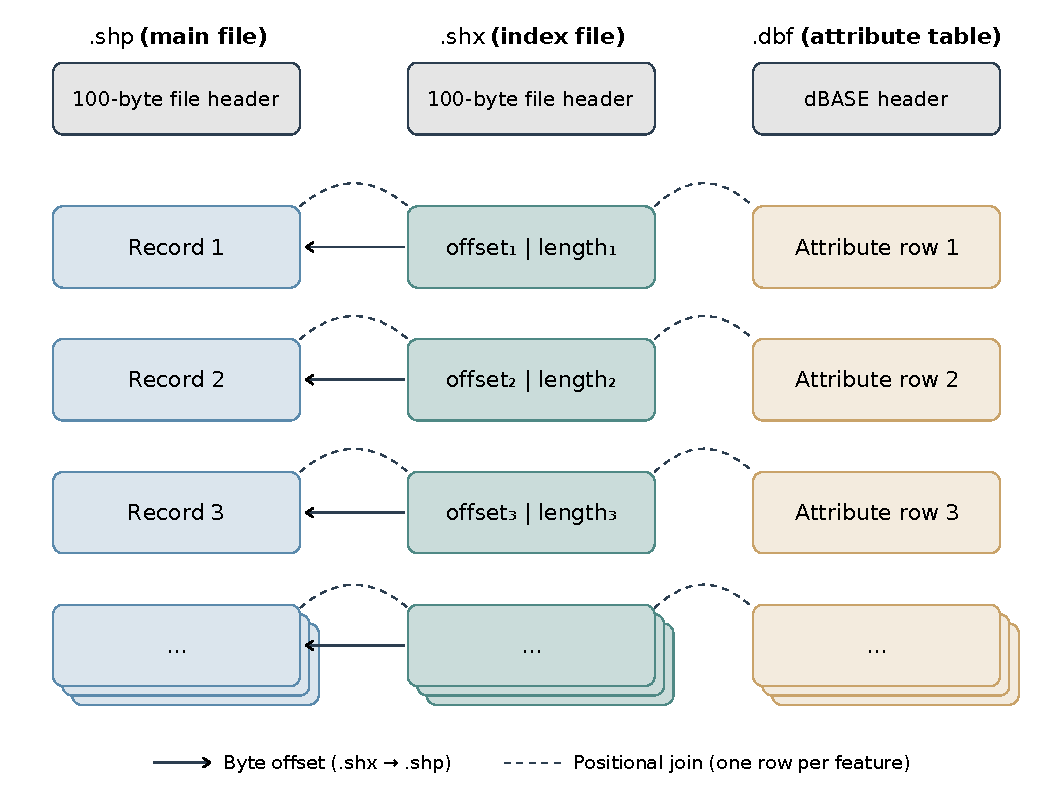
\includegraphics[width=0.7\textwidth]{Chapters/02-background/sub-chapters/figures/02-shapefile-linkage.pdf}
    \caption[Component-file linkage in a Shapefile]{Component-file linkage in a Shapefile. Each entry in the \texttt{.shx} index points (solid arrow) to the byte offset of the corresponding variable-length record in the \texttt{.shp} main file. The \texttt{.dbf} attribute table holds one row per feature in the same order as the \texttt{.shp} records, so attributes and geometries are joined by record position rather than by a key column (dashed connectors). Adapted from \textcite{esri1998_shapefile_technical_description}.}
    \label{fig:shapefile-linkage}
\end{figure}

A Shapefile is restricted to a single geometry type per file, chosen from \num{14} values that include 2D, 3D, and measured variants of points, polylines, polygons, and multipoints \parencite{esri1998_shapefile_technical_description}. The format records no topology, the explicit characterization of spatial relationships and shared geometry between features \parencite{ogc2007_07036_gml_specification}. The original specification also defines no \acrshort{crs}, and this information is supplied instead through an auxiliary \acrshort{wkt} file that emerged as a de facto convention with later \acrshort{esri} products \parencite{esri1998_shapefile_technical_description, gdal2025_shapefile_driver}.

The \texttt{.shx} index provides direct access to any feature record by byte offset, but it is a record index rather than a spatial index, and cannot accelerate bounding-box or intersection queries. A spatial index must be created separately and stored in one of the auxiliary files in Table~\ref{tab:shapefile-components}, either \acrshort{esri}'s undocumented \texttt{.sbn}/\texttt{.sbx} files or the quadtree \texttt{.qix} files used by MapServer and \acrfull{gdal} \parencite{gdal2025_shapefile_driver}. Without such an index, evaluating a spatial predicate requires a sequential scan of the \texttt{.shp} file, reading and parsing every record in order, since the format carries no per-record or per-block metadata that would let a reader skip features without first reading them.

% Academic rewrite
The format also imposes constraints on file size and value representation. The \texttt{.shp} file addresses its records through \num{32}-bit offsets counted in \num{16}-bit words \parencite{esri1998_shapefile_technical_description}, so the format itself tops out near \num{8}~GB, with the \acrshort{gdal} implementation capping it lower at \num{4}~GB \parencite{gdal2025_shapefile_driver}. In practice a \num{2}~GB size limit applies to each component file for compatibility across software \parencite{esri2024_arcmap_shapefile_output}, so datasets exceeding this size must be partitioned across multiple Shapefiles. Floating-point values are stored as text rather than binary, which can introduce rounding errors on read and write \parencite{esri2024_arcmap_shapefile_output}, and the format has no native representation of \texttt{null}: \acrshort{esri} software writes null values as zero \parencite{esri2024_arcmap_shapefile_output}.

\subsubsection{GeoJSON}
\label{background:spatial-data-formats-and-storage-models:file-formats:geojson}
GeoJSON is a text-based format for geographic data based on \acrfull{json}. The \acrfull{ietf} standardized it as \acrfull{rfc}~7946 in August 2016, replacing a 2008 community specification \parencite{butler2016_rfc7946_geojson_format}. Its \acrfull{iana} media type\footnote{A media type is a standardized label for the format of a resource, registered with \acrshort{iana}, that allows software to recognize how the content should be processed.} is \texttt{application/geo+json}, with file extensions \texttt{.json} or \texttt{.geojson} \parencite{butler2016_rfc7946_geojson_format}.

A GeoJSON document is a single \acrshort{json} object whose type is one of the seven \acrshort{ogc} Simple Features geometry types or one of two wrappers unique to GeoJSON. A \texttt{Feature} pairs a geometry with a \texttt{properties} object holding its attributes, and a \texttt{FeatureCollection} is a list of features. Unlike Shapefile's \texttt{.shp}/\texttt{.dbf} pairing, geometries and attributes are stored together and parsed as a single unit \parencite{butler2016_rfc7946_geojson_format}.

Coordinates are \acrshort{json} arrays of two or three numbers: longitude, latitude, and optional altitude. Implementations should not use more than three elements \parencite{butler2016_rfc7946_geojson_format}. \acrshort{rfc}~7946 requires all coordinates to be in WGS84 longitude and latitude (\texttt{OGC:CRS84}), removing support for alternative reference systems that caused interoperability problems \parencite{butler2016_rfc7946_geojson_format}. The standard also mandates the right-hand rule for polygon rings, a winding convention in which exterior rings run counterclockwise and holes clockwise to identify each ring's interior. For bounding boxes it uses \texttt{[west, south, east, north]} rather than \texttt{minx, miny, maxx, maxy} \parencite{butler2016_rfc7946_geojson_format}.

GeoJSON has no indexing mechanism. Unlike Shapefile's \texttt{.shx}, it lacks structures for fast access, row-group statistics, or embedded metadata identifying byte ranges. Any query, spatial or attribute-based, therefore requires parsing every Feature from the start of the file, because a \acrshort{json} parser cannot skip Features and must tokenize the entire document, scanning each character to recognize the structural delimiters that mark Feature boundaries. The \texttt{type} field may appear only after a long \texttt{features} array, so large files must be read in full before their structure can be confirmed \parencite{butler2016_rfc7946_geojson_format}.

GeoJSON is plain text and readable by any tool that supports \acrshort{json}, which has made it popular for web maps, \acrshort{json}-based \acrshort{api}s, and ad hoc data exchange. At scale, these same properties become limitations. Files cannot be partially parsed, which forces the entire document to be downloaded before use and makes the format unsuitable for cloud-optimized access \parencite{cngfoundation2024_cloud_optimized_geospatial_formats_guide}.

\subsubsection{Geography Markup Language}
\label{background:spatial-data-formats-and-storage-models:file-formats:geography-markup-language}
\acrfull{gml} is an \acrfull{xml}-based format for geographic information, standardized as \acrshort{ogc} 07-036 and \acrfull{iso} 19136:2007 \parencite{ogc2007_07036_gml_specification}. A \acrshort{gml} dataset is defined by a schema together with an instance document, which makes it less self-contained than GeoJSON or Shapefile \parencite{ogc2007_07036_gml_specification}. Its geometry model extends beyond Simple Features to non-linear curves, solids, and topology primitives \parencite{ogc2007_07036_gml_specification}. The format defines no native index \parencite{lu2005_advances_in_gml_geospatial_applications} and uses a verbose, text-based encoding \parencite{guo2010_effective_gml_documents_compressor}, so large datasets are impractical to query in place and are typically loaded into a spatial database for analysis \parencite{li2004_gml_storage_spatial_database}. \acrshort{gml} remains the default encoding for most data specifications under the European \acrfull{inspire} framework \parencite{ec2010_commission_regulation_1089_inspire, inspire2023_d27_encoding_guidelines}.

\subsubsection{GeoParquet}
\label{background:spatial-data-formats-and-storage-models:file-formats:geoparquet}
GeoParquet stores geospatial data in Apache Parquet, a widely adopted columnar file format for analytical workloads \parencite{ogc2024_geoparquet_specification_v110, lamb2022_querying_parquet_millisecond_latency}. Its cloud-native properties follow from Parquet itself, not from any geospatial extension, and reflect the broader shift from row-oriented to columnar storage in modern data platforms.

GeoParquet files follow Parquet's internal structure, illustrated in Figure~\ref{fig:geoparquet-file-format}. Rows are organized into row groups, contiguous and independently readable partitions, and within each group every column is stored separately so that a query touches only the columns it needs. The file footer holds a metadata index with the location and min/max statistics of every column in every row group \parencite{lamb2022_querying_parquet_millisecond_latency}. Geometries occupy a binary column encoded either in \acrshort{wkb} or in GeoArrow, a columnar alternative to WKB, so per-group statistics extend to geometry as well \parencite{ogc2024_geoparquet_specification_v110}.

\begin{figure}[H]
    \centering
    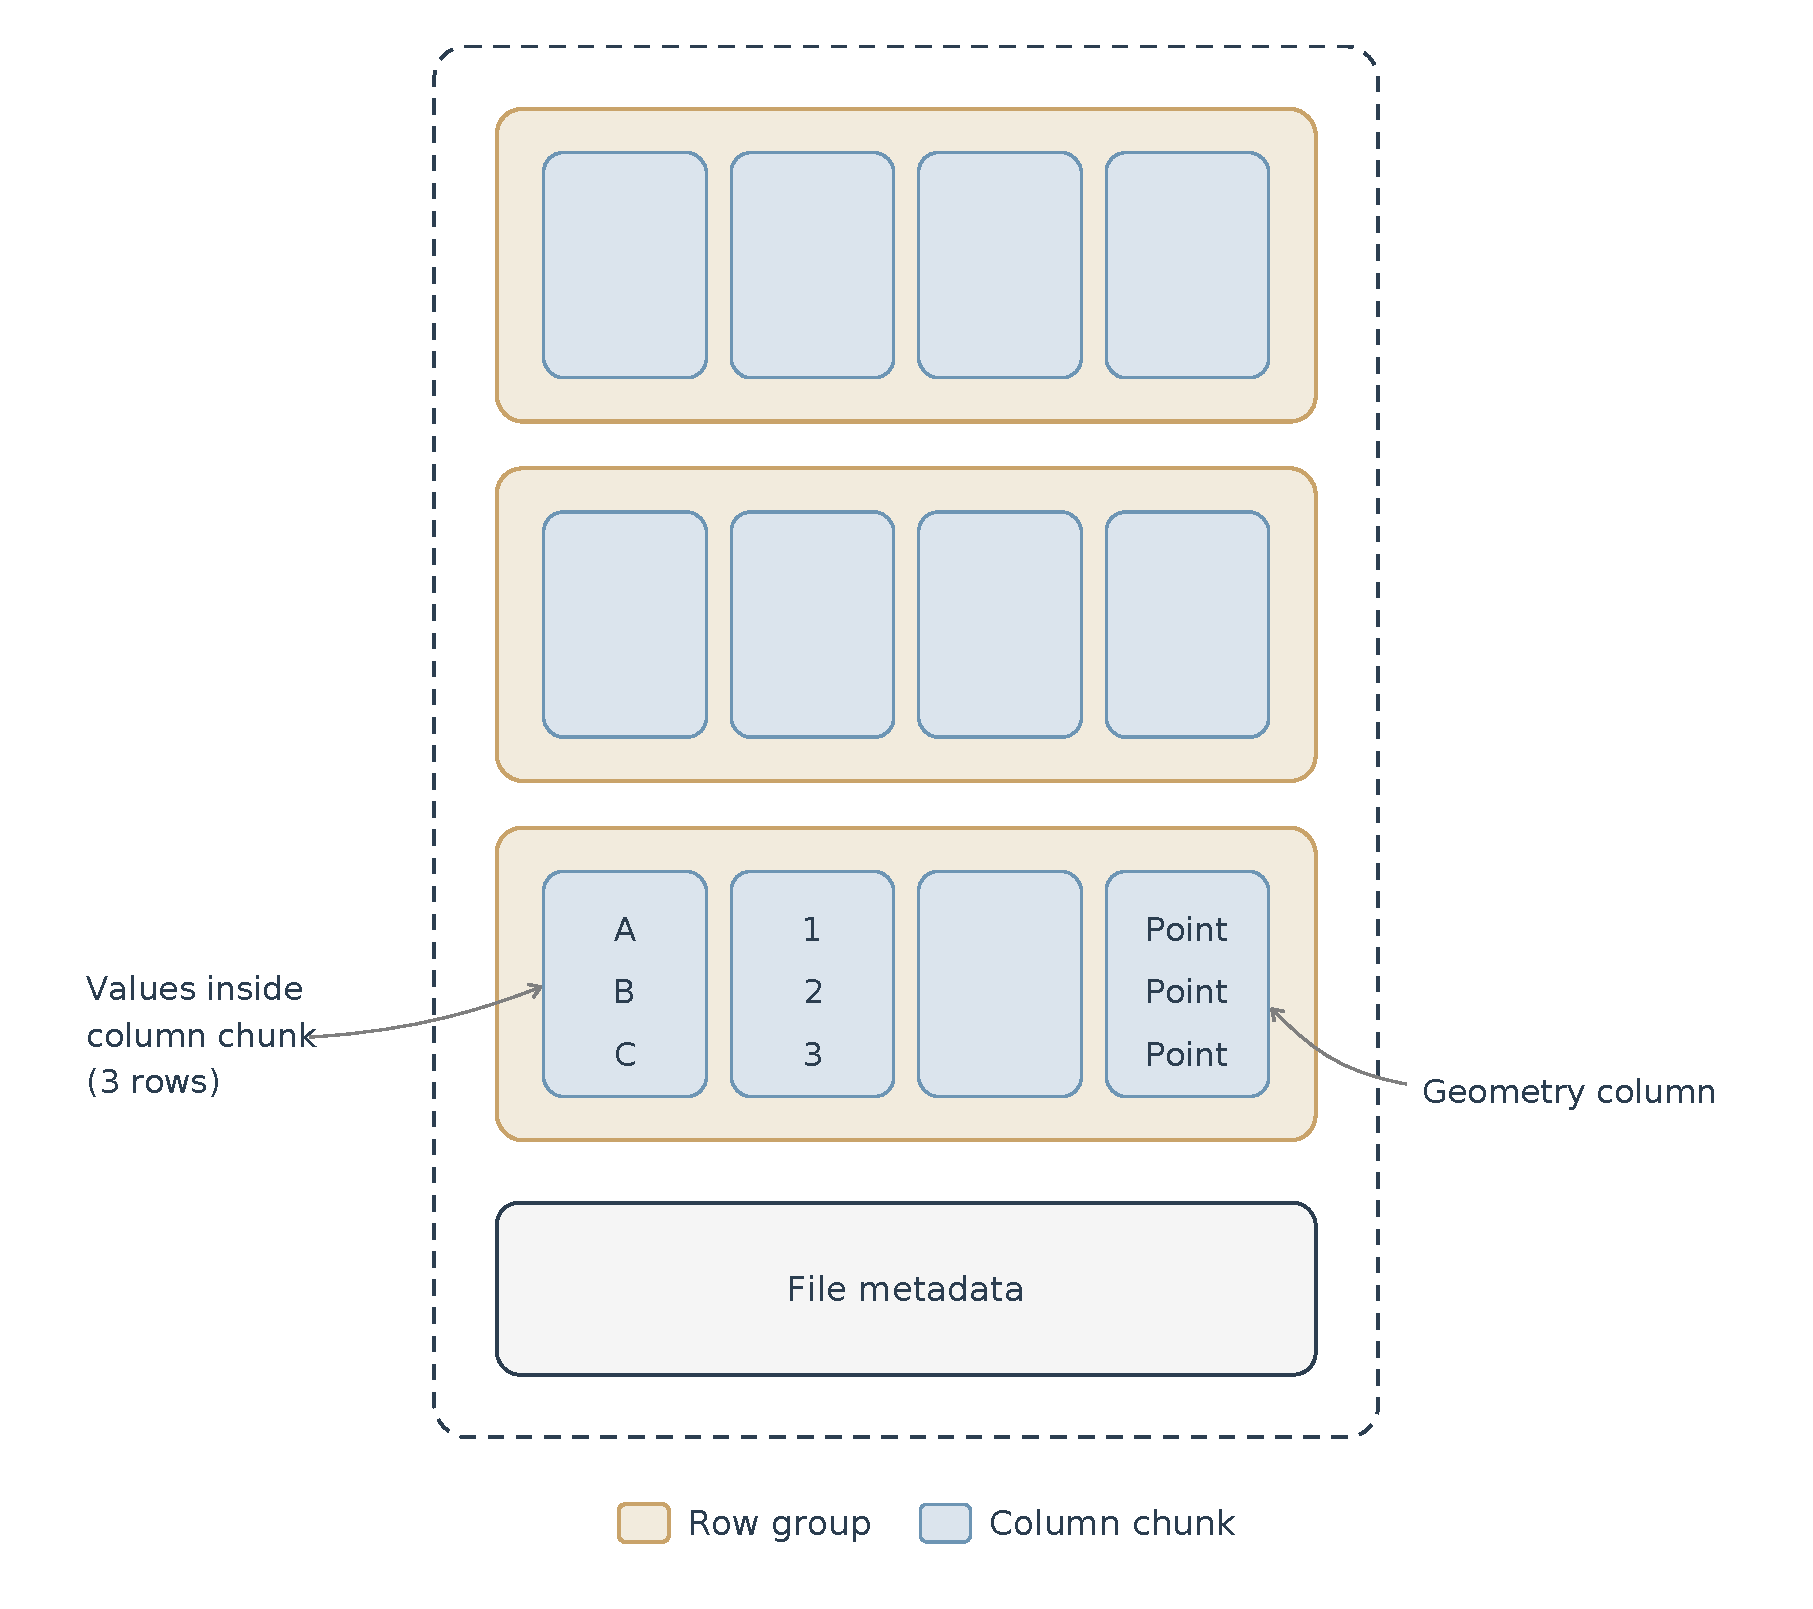
\includegraphics[width=0.75\textwidth]{Chapters/02-background/sub-chapters/figures/02-geoparquet-file-format.pdf}
    \caption[Internal structure of a GeoParquet file]{Internal structure of a GeoParquet file. Rows are grouped into row groups, each holding one column chunk per column, and the file footer holds the metadata index with location and min/max statistics for every column chunk. Adapted from \textcite{cngfoundation2024_geoparquet_guide}.}
    \label{fig:geoparquet-file-format}
\end{figure}

Coordinate reference systems are described in PROJJSON, a \acrshort{json} encoding of WKT2:2019, with \texttt{OGC:CRS84} (WGS84 longitude and latitude) as the default when none is specified \parencite{ogc2024_geoparquet_specification_v110}. The specification also fixes axis order to \texttt{(x, y)} regardless of the \acrshort{crs}, avoiding the latitude/longitude ambiguity that affects \acrshort{gml} \parencite{ogc2024_geoparquet_specification_v110}.

The format is built for selective reads. By comparing query predicates against each row group's min/max statistics in the footer, a reader can skip groups whose values cannot satisfy the predicate, an optimization known as predicate pushdown \parencite{lamb2022_querying_parquet_millisecond_latency}. The columnar layout further enables projection pushdown, so a reader fetches only the columns the query references \parencite{lamb2022_querying_parquet_millisecond_latency}. GeoParquet 1.1 extends this pruning to spatial predicates through an optional per-row bounding-box encoding with \texttt{xmin}, \texttt{ymin}, \texttt{xmax}, \texttt{ymax} columns, so spatial filters benefit from the same row-group skipping as scalar filters \parencite{ogc2024_geoparquet_specification_v110}. Although Parquet was designed for \acrfull{hdfs}, its access pattern transfers to commodity object storage because the two share similar performance characteristics \parencite{lamb2022_querying_parquet_millisecond_latency}. Readers therefore issue \acrshort{http} range requests for the footer and the row groups they need, leaving the rest of the file untransferred \parencite{cngfoundation2024_cloud_optimized_geospatial_formats_guide}.

The limitations follow from the same static columnar design. Parquet files are immutable, so any update or append requires rewriting the file in full \parencite{microsoft2024_direct_lake_parquet_immutability}. Workloads dominated by many small files also suffer, because each open incurs a separate footer fetch \parencite{cngfoundation2024_geoparquet_guide}. The format defines no spatial index proper; the 1.1 bounding-box covering enables row-group pruning but cannot stand in for an R-tree on complex joins or nearest-neighbor searches \parencite{cngfoundation2024_geoparquet_guide}. The geometry model is also narrower than some alternatives, omitting M values and non-linear geometry types and requiring geometry to sit as a top-level column rather than a nested field \parencite{ogc2024_geoparquet_specification_v110}. For best results, the specification recommends row groups of \numrange{50000}{150000} rows, spatial partitioning of files larger than \num{2}~GB, and compression with zstd, a general-purpose codec that balances speed and ratio \parencite{ogc2024_distributing_geoparquet}.

\subsection{File databases}
\label{background:spatial-data-formats-and-storage-models:file-databases}
A file database is a single, portable file that bundles the data, an embedded query engine, and indexes. Unlike a flat file, it answers queries using its own indexes. Unlike a server-based engine, in which a long-running server process accepts client queries and arbitrates concurrent access, a file database needs no such process. The engine is linked into the calling application as a library and reads the file through ordinary function calls, so file databases are easy to deploy and move between machines. The trade-off is write concurrency, the ability for multiple writers to modify the data simultaneously. With no server to arbitrate access, the database falls back on file-level coordination through operating-system file locks, which limits how many writers can operate at once. File databases therefore serve single-user analysis and data exchange well, but not workloads with many concurrent writes.

SpatiaLite and \acrshort{ogc} GeoPackage both build on SQLite, a public-domain, in-process \acrfull{sql} engine whose database is a single cross-platform file \parencite{sqlite2024_about, gaia2011_spatialite_manual, ogc2024_geopackage_encoding_standard_140}. Both store geometries in BLOB columns and index them with SQLite's R*Tree module \parencite{gaia2011_blob_geometry, sqlite2024_rtree_module, ogc2024_geopackage_encoding_standard_140}. The \acrshort{esri} \acrfull{fgdb} instead packages each table as binary files in a \texttt{.gdb} folder and indexes geometry with a proprietary grid-based structure whose layout is known publicly only through reverse engineering \parencite{rouault2013_filegdb_format_specification, gdal2025_openfilegdb_driver}. All three embed the engine in the file and coordinate access through file-level locks, so they share SQLite's single-writer constraint and are unsuited to network file systems or high-concurrency writes \parencite{sqlite2024_appropriate_uses}. None supports selective reads from object storage over \acrshort{http}, the property that defines the cloud-native tier, so no file-database configuration enters the benchmark.

\subsection{Full database engines}
\label{background:spatial-data-formats-and-storage-models:full-database-engines}
A full database engine stores spatial data in tables managed by a query engine that supports a query language, typically SQL, and treats concurrency, transactions, and indexing as first-class concerns, meaning the engine implements them directly rather than leaving them to the application. Two architectural patterns dominate. In the client/server model, exemplified by PostgreSQL, a long-running server process manages the database files and accepts connections from client applications. For each connection the server forks a new backend process, a separate operating-system process spawned on demand to serve that client, so that many clients can read and write concurrently \parencite{postgresql2024_architectural_fundamentals}. Concurrent access is coordinated through \acrfull{mvcc}, which gives each statement a consistent snapshot of the data without blocking readers behind writers \parencite{postgresql2024_concurrency_control}. In the in-process model, exemplified by DuckDB, the engine is a library linked into the calling application; there is no separate server process, and queries run in the application's own address space, the memory region the operating system allocates to a single running process \parencite{raasveldt2019_duckdb_embeddable_analytical_database}. The two models couple the query engine to the data alike, but make different trade-offs around concurrency, deployment, and the path between storage and compute. The two systems described next realize these patterns.

\subsubsection{PostGIS}
\label{background:spatial-data-formats-and-storage-models:full-database-engines:postgis}
PostGIS is an open-source extension for PostgreSQL that adds spatial types, functions, and indexes \parencite{postgis2024_manual_34}. An extension here is a loadable module that PostgreSQL registers through its own catalog, so installed extensions behave as native parts of the database. The user enables it with \texttt{CREATE EXTENSION postgis}, and optional companion extensions add raster, topology, and SFCGAL-based 3D operations \parencite{postgis2024_manual_34}. Because PostGIS sits inside PostgreSQL, it inherits the database's transactional machinery: \acrshort{mvcc} concurrency control, which gives every statement a consistent snapshot of the data so readers never block writers \parencite{postgresql2024_concurrency_control}, \acrshort{wal}-based crash recovery \parencite{postgresql2024_wal}, and \acrfull{rbac} \parencite{postgresql2024_roles}. The extension reads and writes a broad set of formats, including \acrshort{wkt}, \acrshort{wkb}, \acrshort{ewkt}, \acrshort{ewkb}, GeoJSON, \acrshort{gml}, \acrfull{kml}, and \acrfull{svg}, which keeps it interoperable with most geospatial tools \parencite{postgis2024_manual_34}.

Unlike the formats discussed earlier in this chapter, PostGIS defines no file layout of its own. Spatial data resides in ordinary PostgreSQL tables \parencite{postgis2024_manual_34} and is managed by a long-running server process \parencite{postgresql2024_architectural_fundamentals}. To comply with the \acrshort{ogc} Simple Features for \acrshort{sql} specification, the extension maintains two metadata tables: \texttt{spatial\_ref\_sys}, which registers coordinate reference systems, and \texttt{geometry\_columns}, which records each spatial table's geometry column \parencite{postgis2024_manual_34}.

PostGIS exposes two spatial types built on different geometric models. The core \texttt{GEOMETRY} type stores planar geometry in any coordinate system identified by SRID and supports the full \acrshort{ogc} Simple Features geometry set, including M, Z, and ZM variants \parencite{postgis2024_manual_34}. The \texttt{GEOGRAPHY} type targets geodetic computation: it accepts any longitude/latitude-based \acrshort{srs}, returns measurements in meters, and covers a smaller geometry set that excludes curves, \acrlong{tin}s (\acrshort{tin}), and polyhedral surfaces \parencite{postgis2024_manual_34}. A large library of geometry-processing functions complements these types, with further capability added through the raster, topology, and SFCGAL extensions \parencite{postgis2024_manual_34}.

Spatial indexing in PostGIS builds on PostgreSQL's \acrshort{gist} framework, with an R-tree as the default spatial access method \parencite{postgis2024_manual_34, hellerstein1995_generalized_search_trees_database_systems}. \acrshort{gist} is an extensible structure that hosts B+-trees, R-trees, and other tree-based indexes behind a common set of operations \parencite{hellerstein1995_generalized_search_trees_database_systems}. PostGIS also supports \acrfull{spgist} indexes for quadtrees and k-d trees, and \acrfull{brin} indexes, which store per-block summary statistics rather than per-row entries and suit read-mostly data \parencite{postgis2024_manual_34}. Only bounding-box-based operators use the spatial index directly; functions such as \texttt{ST\_Distance} benefit from the index only when a bounding-box predicate is also supplied \parencite{postgis2024_manual_34}.

PostGIS's main limitation for cloud deployments is architectural rather than one of scale. Storage and compute are tightly coupled in the PostgreSQL model \parencite{dageville2016_snowflake_elastic_data_warehouse}: all data must be loaded into the server, and every query executes inside the server process \parencite{postgresql2024_architectural_fundamentals}, which makes PostGIS a poor fit for workflows that read directly from object storage \parencite{pang2024_storage_disaggregated_databases}. Client connections are likewise mediated by the server \parencite{postgresql2024_architectural_fundamentals}. Scaling out across machines therefore requires either replication, copying the data to additional servers, or sharding, partitioning the data across servers so each holds a subset \parencite{stonebraker1986_case_for_shared_nothing}. Cloud-native file formats, by contrast, let many compute processes read the same file directly from object storage without routing through a central server.

\subsubsection{DuckDB with the spatial extension}
\label{background:spatial-data-formats-and-storage-models:full-database-engines:duckdb-with-the-spatial-extension}
DuckDB is an in-process database management system for analytical workloads, much as SQLite serves transactional workloads dominated by small individual reads and writes \parencite{raasveldt2019_duckdb_embeddable_analytical_database}. Applications embed the engine and run queries in their own process, with no separate server required \parencite{raasveldt2019_duckdb_embeddable_analytical_database}. Its \acrshort{sql} dialect resembles PostgreSQL \parencite{duckdb2025_sql_introduction}. Spatial support is added by the \texttt{spatial} extension, which provides a \texttt{GEOMETRY} type based on the \acrshort{ogc} Simple Features model and integrates GEOS, \acrshort{gdal}, and PROJ for algorithms, format conversion, and coordinate transformation \parencite{gabrielsson2023_postgeese_duckdb_spatial_extension, duckdb2025_spatial_extension_overview}.

Like PostGIS, DuckDB does not define a file layout for spatial data. Tables loaded into DuckDB, known as managed tables, sit in the engine's own internal storage format, which partitions them into compressed column blocks and tracks per-block minimum and maximum statistics so that irrelevant blocks are skipped at query time \parencite{raasveldt2019_duckdb_embeddable_analytical_database}. Execution is vectorized: rather than processing one row at a time, query operators such as scans, filters, joins, and aggregations operate on fixed-size column-oriented containers called Vectors \parencite{duckdb2025_vector}. DuckDB can also operate directly on external files. The \texttt{httpfs} extension enables reading Parquet and other supported formats from \acrshort{http}, S3, Google Cloud Storage, and similar object storage \parencite{duckdb2025_documentation_httpfs}. Through \acrshort{gdal}, the spatial extension supports over \num{50} vector formats via the \texttt{ST\_Read} table function, so formats such as Shapefile, GeoPackage, or GeoJSON can be queried directly with \acrshort{sql} without explicit import \parencite{gabrielsson2023_postgeese_duckdb_spatial_extension}.

The core spatial type is \texttt{GEOMETRY}, based on the \acrshort{ogc} Simple Features model, and a large library of \texttt{ST\_}-prefixed functions handles geometry processing, format conversion, and coordinate transformation \parencite{gabrielsson2023_postgeese_duckdb_spatial_extension, duckdb2025_spatial_extension_overview}. From version 1.5, \texttt{GEOMETRY} became a built-in DuckDB type, though its functions remain in the spatial extension \parencite{duckdb2025_spatial_extension_overview}. The extension also includes experimental columnar native types such as \texttt{POINT\_2D} and \texttt{POLYGON\_2D}, which trade flexibility for better compression and faster execution \parencite{gabrielsson2023_postgeese_duckdb_spatial_extension, duckdb2025_spatial_extension_overview}.

{\sloppy
Spatial indexing in DuckDB uses an R-tree whose leaf nodes store the approximate minimum bounding rectangle of each geometry. The index is consulted when the query filter includes intersection-implying predicates such as \texttt{ST\_Intersects}, \texttt{ST\_Within}, or \texttt{ST\_Contains} \parencite{duckdb2025_spatial_extension_rtree_indexes}. DuckDB also keeps automatic min/max indexes for general-purpose data types, which act as zonemaps for predicate pruning \parencite{duckdb2025_documentation_indexes}. For Parquet files, DuckDB supports both projection and predicate pushdown to remote sources, reading only the required columns and skipping row groups that do not match the filter \parencite{duckdb2025_parquet_overview, duckdb2025_documentation_httpfs}.
\par}

DuckDB combines an in-process query engine, a Simple Features geometry type, and direct access to object storage, placing it between traditional and cloud-native systems. It offers a \acrshort{sql} interface and transactional behavior but can also operate on cloud-native files in object storage without loading them into managed tables. DuckDB is a single-node engine and scales vertically by adding resources to one machine rather than horizontally by distributing work across nodes \parencite{duckdb2025_scalability_faq}. Workloads that exceed one machine cannot be handled by adding more DuckDB nodes. Current limitations of the spatial extension include no spherical geometry, no Z or M dimensions in \texttt{GEOMETRY}, and no support for curve or polyhedral-surface types \parencite{gabrielsson2023_postgeese_duckdb_spatial_extension, duckdb2025_spatial_extension_overview}.

The two database engines compared above share a common foundation: a \acrshort{sql} query engine, an \acrshort{ogc} Simple Features geometry type, and R-tree spatial indexing. They differ in architecture. PostGIS runs as a server-based extension to PostgreSQL and scales vertically or through replication and sharding. DuckDB is an in-process single-node engine that can also read cloud-native files in object storage directly.

\subsection{In-memory dataframe libraries}
\label{background:spatial-data-formats-and-storage-models:in-memory-dataframe-libraries}

A fourth model reads spatial data into program memory and operates on it there, with no embedded query engine and no separate server process. In the Python ecosystem its established representative is GeoPandas \parencite{jordahl2024_geopandas}, which extends the pandas dataframe \parencite{mckinney2010_data_structures_statistical_computing} with a geometry column. A table of features then becomes a \texttt{GeoDataFrame} held entirely in the address space of the calling process, and analysis proceeds by calling library functions on that object rather than by issuing queries to an engine. Geometry operations are delegated to Shapely, the default backend since GeoPandas 0.14, which exposes the GEOS geometry library \parencite{geopandas2024_pygeos_to_shapely}. Fiona or pyogrio handle file \acrshort{io} over \acrshort{gdal}, and pyproj handles coordinate transformation over PROJ \parencite{jordahl2024_geopandas}.

Like the database engines, GeoPandas defines no on-disk format of its own. It reads and writes through the \acrshort{gdal} driver stack, and through the pyarrow library for GeoParquet and Feather, the columnar formats built on Apache Arrow \parencite{geopandas2024_reading_and_writing_files}. By default, a read materializes an entire layer into memory as a \texttt{GeoDataFrame} \parencite{geopandas2024_reading_and_writing_files, geopandas2024_read_file}. The reader can narrow what is loaded by passing a bounding box or geometry mask, a row slice, a column subset, or an \acrshort{sql} attribute filter, each delegated to the \acrshort{gdal} engine, but these filters are opt-in \parencite{geopandas2024_reading_and_writing_files, geopandas2024_read_file}. Shapely 2.0 vectorizes geometry operations, applying GEOS to the whole array of geometries at once rather than processing one geometry at a time in Python \parencite{geopandas2024_pygeos_to_shapely}.

GeoPandas keeps no persistent spatial index. On first access to the \texttt{.sindex} property, it builds an in-memory R-tree, the Sort-Tile-Recursive tree provided by Shapely, and caches it on the object \parencite{geopandas2024_spatial_indexing}. The spatial join, overlay, and clip operations consult this index automatically, whereas an elementwise predicate such as testing intersection against a single geometry does not, instead testing every geometry in turn \parencite{geopandas2024_spatial_indexing}.

Because the dataset occupies the memory of a single process, GeoPandas scales only vertically, by enlarging that machine, and the core library spills nothing to disk. The separate dask-geopandas project provides distributed or larger-than-memory execution \parencite{geopandas2024_dask_geopandas}. GeoPandas maintains no managed-table storage, no transactions, and no concurrency control. It therefore embodies the traditional read model, in which analysis begins by materializing the full dataset in memory \parencite{jordahl2024_geopandas}, in contrast to the selective, range-based reads the cloud-native formats support. This memory ceiling bounds the dataset size GeoPandas can process.

\subsection{Summary}
\label{background:spatial-data-formats-and-storage-models:summary}

% Academic rewrite
The formats and engines in this section fall into three architectural tiers: flat files, file databases, and full database engines. Table~\ref{tab:format-summary} compares them along three dimensions that shape benchmark outcomes --- native spatial indexing, primary access pattern, and support for cloud-native access through \acrshort{http} range requests on object storage --- with horizontal rules separating the tiers in the order introduced. Of these, four carry into the remainder of the thesis: Shapefile as the representative legacy flat file, read with the GeoPandas in-memory dataframe library described in Section~\ref{background:spatial-data-formats-and-storage-models:in-memory-dataframe-libraries}; GeoParquet as the cloud-native flat file; and two full database engines, the server-based PostGIS and the in-process DuckDB, whose cloud-native access is realised specifically when it reads GeoParquet over object storage --- the configuration used in the benchmark.

\begin{table}[H]
    \centering
    \footnotesize
    \setlength{\tabcolsep}{6pt}
    \renewcommand{\arraystretch}{1.2}
    \caption[Summary of spatial data formats and engines]{Spatial data formats and engines compared along the dimensions used in this thesis.}
    \label{tab:format-summary}
    \begin{tabularx}{\textwidth}{@{}l L L c@{}}
        \toprule
        \textbf{Format / engine} & \textbf{Native spatial index} & \textbf{Access pattern} & \textbf{Cloud-native} \\
        \midrule
        Shapefile         & Optional sidecar           & Sequential scan                       & No      \\
        GeoJSON           & None                       & Full parse                            & No      \\
        \acrshort{gml}    & None                       & Full parse                            & No      \\
        GeoParquet        & Optional bbox covering     & Range requests, pushdown              & Yes     \\
        \midrule
        SQLite/SpatiaLite & R*Tree                     & Engine through file                   & No      \\
        GeoPackage        & R*Tree                     & Engine through file                   & No      \\
        File Geodatabase  & Grid-based (proprietary)   & Engine through files                  & No      \\
        \midrule
        PostGIS           & R-tree on \acrshort{gist}  & Server-mediated \acrshort{sql}        & No      \\
        DuckDB + spatial  & R-tree                     & In-process \acrshort{sql} or remote   & Partial \\
        \bottomrule
    \end{tabularx}
\end{table}